%******************************************************************************%
% Copyright (C) 2018  Louis Solofrizzo                                         %
%                                                                              %
% This content is considered a free software: you can redistribute it          %
% and/or modify it under the terms of the GNU General Public License as        %
% published by the Free Software Foundation, either version 3 of the License,  %
% or (at your option) any later version.                                       %
%                                                                              %
% This program is distributed in the hope that it will be useful,              %
% but WITHOUT ANY WARRANTY; without even the implied warranty of               %
% MERCHANTABILITY or FITNESS FOR A PARTICULAR PURPOSE.  See the                %
% GNU General Public License for more details.                                 %
%                                                                              %
% You should have received a copy of the GNU General Public License            %
% along with this program.  If not, see <https://www.gnu.org/licenses/>.       %
%******************************************************************************%

%******************************************************************************%
%                                                                              %
%                          KFS_1.en.tex for KFS_1                              %
%                                                                              %
%                  Created on : Wed May 25 13:27:28 2016                       %
%          Made by : Louis "Ne02ptzero" Solofrizzo <louis@ne02ptzero.me>       %
%                                                                              %
%******************************************************************************%

\documentclass{42-en}


%******************************************************************************%
%                                                                              %
%                                    Prologue                                  %
%                                                                              %
%******************************************************************************%


\begin{document}


                           \title{KFS\_1}
                    \subtitle{Grub, boot and screen}
                    \member{Louis Solofrizzo}{louis@ne02ptzero.me}
                    \member{42 Staff}{pedago@42.fr}

\summary {
	The real code !
}

\maketitle

\tableofcontents


%******************************************************************************%
%                                                                              %
%                                  Forewords                                   %
%                                                                              %
%******************************************************************************%
\chapter{Forewords}
	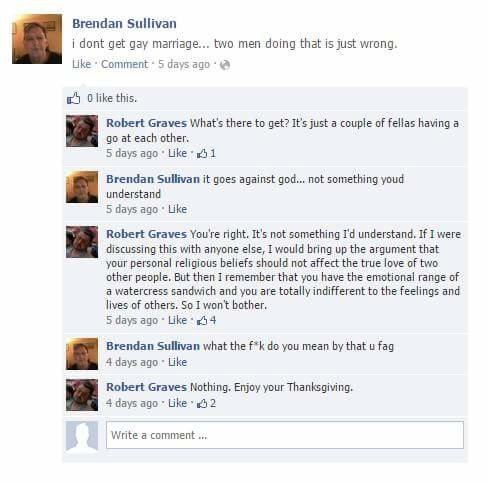
\includegraphics[width=8cm]{bren1.jpg}
	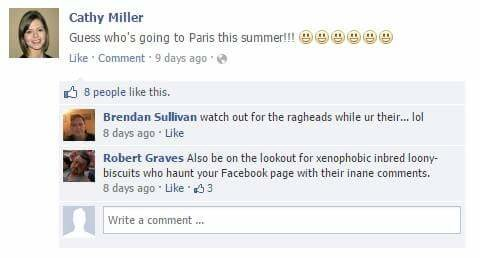
\includegraphics[width=8cm]{bren2.jpg}
	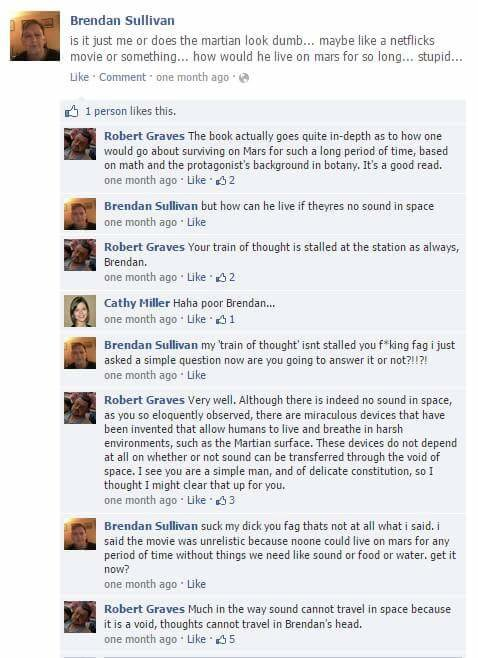
\includegraphics[width=8cm]{bren3.jpg}
	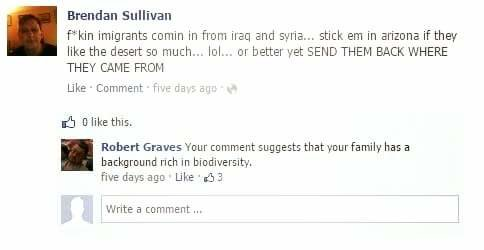
\includegraphics[width=8cm]{bren4.jpg}
	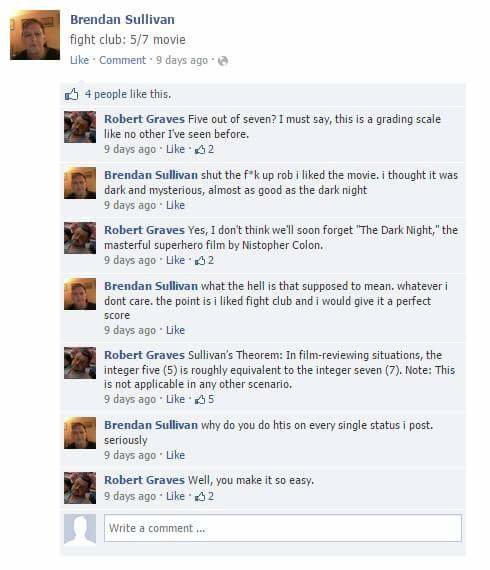
\includegraphics[width=8cm]{bren5.jpg}
	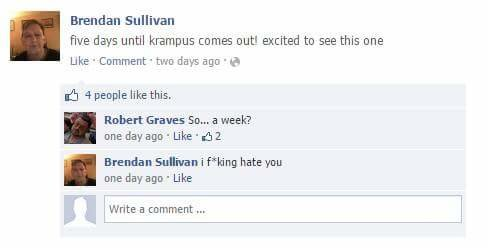
\includegraphics[width=8cm]{bren6.jpg}
	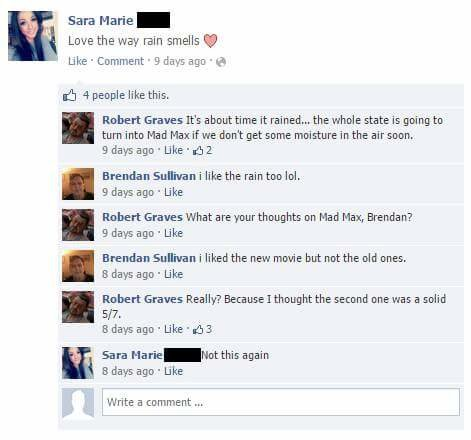
\includegraphics[width=8cm]{bren7.jpg}
	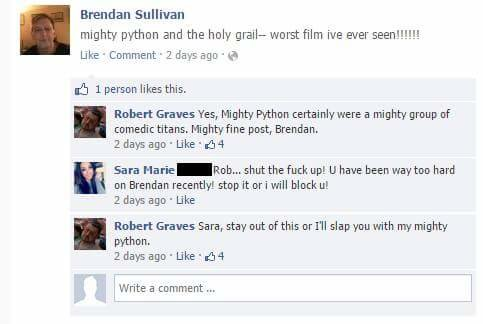
\includegraphics[width=8cm]{bren8.jpg}
	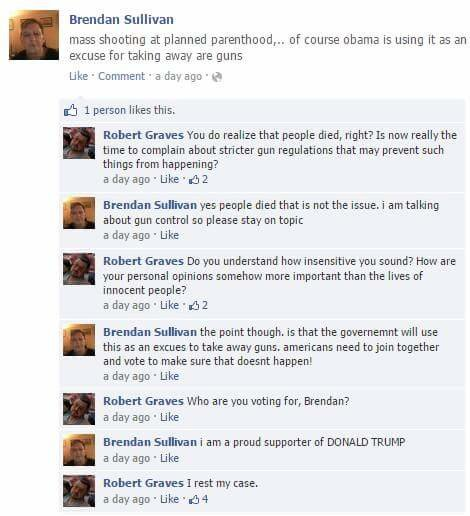
\includegraphics[width=8cm]{bren9.jpg}
	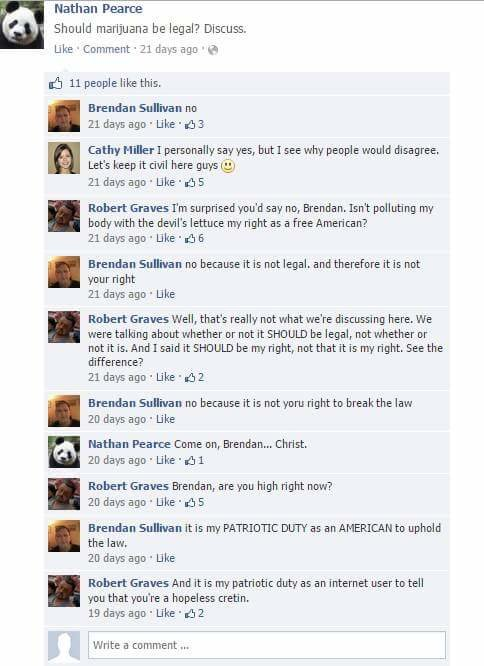
\includegraphics[width=8cm]{bren10.jpg}
	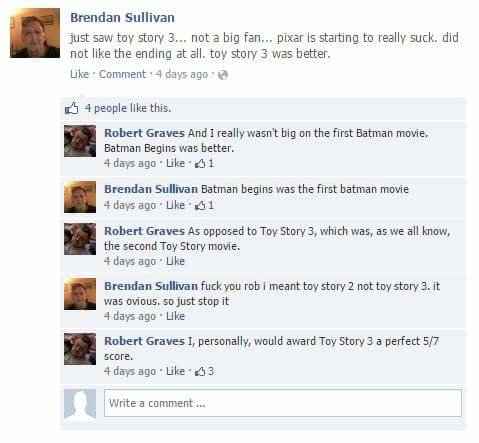
\includegraphics[width=8cm]{bren11.jpg}
	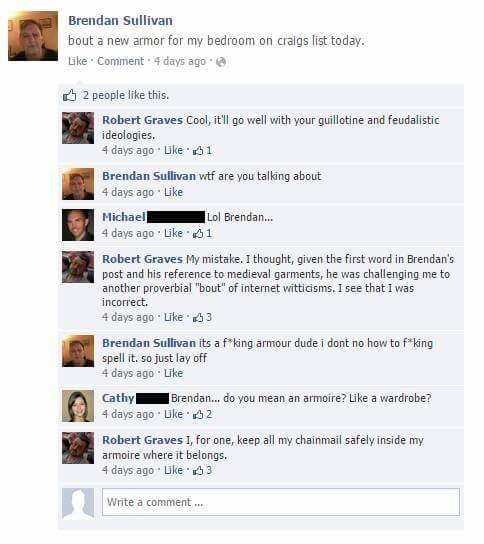
\includegraphics[width=8cm]{bren12.jpg}
	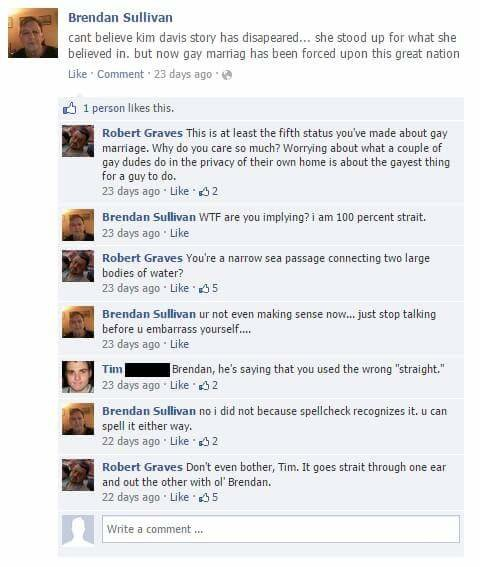
\includegraphics[width=8cm]{bren13.jpg}
	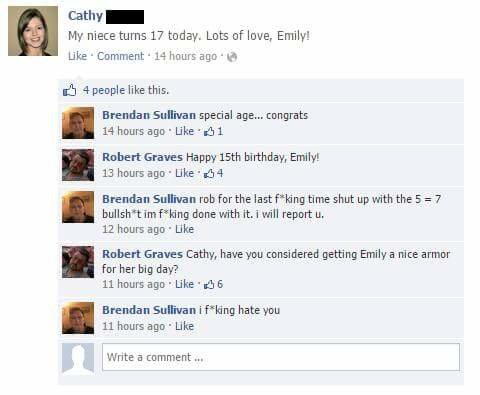
\includegraphics[width=8cm]{bren14.jpg}
	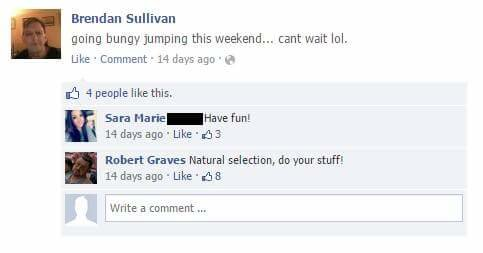
\includegraphics[width=8cm]{bren15.jpg}
	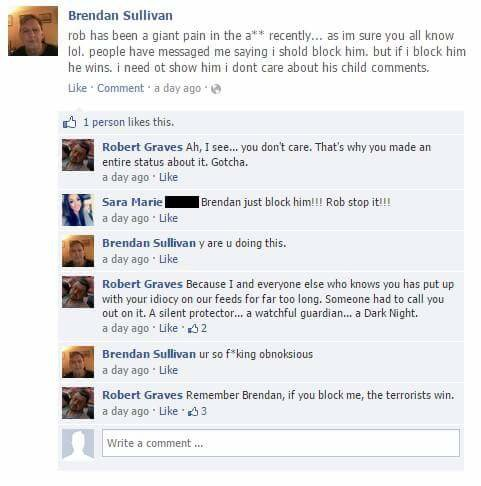
\includegraphics[width=8cm]{bren16.jpg}

\newpage
%******************************************************************************%
%                                                                              %
%                                 Introduction                                 %
%                                                                              %
%******************************************************************************%
\chapter{Introduction}

	Welcome to the first \texttt{Kernel from Scratch} project.\\

	Finally some real coding, I'm pretty sure you were annoyed by the
    Linux Kernel project. In the \texttt{Kernel from Scratch} subjects
    you are going to write a kernel from scratch (no shit ?), without
    any existing software, API, or such.\\

	Once you will be done with those projects and standing on the
    shoulder of your non-revolutionnary-OS, you will be in right to
    laugh at those ordinary Javascript developers, who obviously,
    don't know anything about coding.\\

	On a more serious note, those kernel programming skills are not
    quite spread in the IT world, so \textbf{take your time} to
    understand each and every different points in those projects. One
    does not simply consider himself a 'Kernel developer' if one only
    knows things about drivers or syscalls, like a sysadmin only knows
    things about iptables or softwares installation...  It's a package
    of skills.\\

	A word about the code itself : the \texttt{Kernel From Scratch} is divided into many projects,
    each one dealing with a specific aspect of kernel programming. All
    of those projects are linked together. So when you'll code those
    amazing features, keep in mind that your kernel must be flexible
    and that functions must easily fit in. Half the time you'll spend
    on these projects will be adding links between different aspects
    of your Kernel.\\

	For instance, you must write memory code before processus \& execution code.
	But processus must use memory, right ? So, you gotta link those two !
	So keep your code *clean*, and your internal API simple.\\

	Good luck, and most of all, have fun :)

\newpage
%******************************************************************************%
%                                                                              %
%                                  Goals                                       %
%                                                                              %
%******************************************************************************%
\chapter{Goals}

	At the end of this subject, you will have:

	\begin{itemize}\itemsep1pt
		\item A kernel you can boot via \texttt{GRUB}
		\item An \texttt{ASM} bootable base
		\item A basic kernel library, with basics functions and types
		\item Some basic code to print some stuff on the screen
		\item A basic "Hello world" kernel
	\end{itemize}

	Actually, that's not that much code. This subject is an
    introduction to kernel development. A (wo)man must learn.



\newpage
%******************************************************************************%
%                                                                              %
%                             General instructions                             %
%                                                                              %
%******************************************************************************%
\chapter{General instructions}

	\section{Code and Execution}
		\subsection{Emulation}
			The following part is not mandatory, you are free to use any virtual
			manager you want to, however, i suggest you to use \texttt{KVM}.
			It's a \texttt{Kernel Virtual Manager}, and have advanced execution
			and debugs functions.
			All of the examples below will use \texttt{KVM}.
		\subsection{Language}
			All of \texttt{Kernel from Scratch} subjects have no constraints on
			the language you want to use.\\ 
			C language is not mandatory at all, you can use any language. 
			However, keep in mind that all language are not kernel friendly.
			So... Yes, you could code a Kernel in javascript, but are you sure 
			it's a good idea ?\\
			Also, a lot of example on the documentations are in C, so remember 
			that you will do 'code translation' all the time if you choose a
			different language.\\
			Furthermore, all of the features of a language cannot be used in a
			basic kernel.\\
			Let's take C++ for example:\\
			C++ use 'new' to make allocation, class and structures declaration.
			But in your kernel you do not have a memory interface (yet), so you cannot
			use those features in the beginning.\\
			A lot of language can be used instead of \texttt{C}, like \texttt{C++},
			\texttt{Rust}, \texttt{Go}, etc.
			You could even code your entire kernel in \texttt{ASM} if you want !\\
			So yeah, choose a language, but choose wisely.\\
			\begin{center}
			  
\includegraphics[width=8cm]{choose.jpg}
			\end{center}

\newpage

	\section{Compilation}
		\subsection{Compilers}
			You can choose any compilers you want. I personnaly use	\texttt{gcc}
			and \texttt{nasm}. A Makefile must be turned in.
		\subsection{Flags}
			In order to boot your kernel without any dependencies, you must compile
			your code with the following flags (Adapt the flags for your language,
			those ones are a \texttt{C++} example):
			\begin{itemize}\itemsep1pt
				\item \texttt{-fno-builtin}
				\item \texttt{-fno-exception}
				\item \texttt{-fno-stack-protector}
				\item \texttt{-fno-rtti}
				\item \texttt{-nostdlib}
				\item \texttt{-nodefaultlibs}
			\end{itemize}
			Pay attention to \texttt{-nodefaultlibs} and \texttt{-nostdlib}. 
			Your Kernel will be compiled on a host system, yes, but cannot be 
			linked to any existing library on that host, otherwise it will not 
			be executed.
	\section{Linking}
		You cannot use an existing linker in order to link your kernel.
		As written above, your kernel will not boot. So, you must create a linker
		for your kernel.\\
		Be carefull, you \texttt{CAN} use the 'ld' binary available on your host, 
		but you \texttt{CANNOT} use the .ld file of your host.
	\section{Architecture}
		The i386 (x86) architecture is \texttt{mandatory}
		(you can thank me later).
	\section{Documentation}
		There is a lot of documentation available, good and bad.
		I personnaly think the \texttt{\href{http://wiki.osdev.org/Main_Page}
		{OSDev}} wiki is one of the best.

\newpage
%******************************************************************************%
%                                                                              %
%                             Mandatory part                                   %
%                                                                              %
%******************************************************************************%
\chapter{Mandatory part}

	\subsection{Base}
		You must make a kernel, bootable with \texttt{GRUB}, who can
		write characters on screen.\\
		In order to do that, you have to:
		\begin{itemize}\itemsep1pt
			\item Install \texttt{GRUB} on an virtual image
			\item Write an \texttt{ASM} boot code that handles multiboot
			header,	and use \texttt{GRUB} to init and call main function
			of the kernel itself.
			\item Write basic kernel code of the choosen language.
			\item Compile it with correct flags, and link it to make it bootable.
			\item Once all of those steps above are done, you can write some
			helpers like kernel types or basic functions (strlen, strcmp, ...)
			\item Your work must not exceed 10 MB.
			\item Code the interface between your kernel and the screen.
            \item Display \texttt{"42"} on the screen.
		\end{itemize}
		For the link part, you must create a linker file with the
		\texttt{GNU linker (ld)}. Some docs \href{http://www.math.utah.edu/docs/info/ld_3.html#SEC4}
		{here}.\\

	\subsection{Makefile}
		Your makefile must compile all your source files with the right flags
		and the	right compiler. Keep in mind that your kernel will use at
		least two different	languages (ASM and whatever-you-choose), so make
		(<- joke) your Makefile's rules correctly.\\

		After compilation, all the objects must be linked together in
		order to create	the final Kernel binary (Cf. Linker part).\\

\newpage
%******************************************************************************%
%                                                                              %
%                                 Bonus part                                   %
%                                                                              %
%******************************************************************************%
\chapter{Bonus part}

    Bonus will be evaluated if and only if your mandatory part is
    PERFECT. By PERFECT, I obvioulsy mean that it is complete and
    stable, and free of the tinyest and creepiest error. Actually, if
    your mandatory part is not 100\% on the scale, your bonus will be
    discarded in their ENTIRETY.

	\begin{itemize}\itemsep1pt
		\item Add scroll and cursor support to your I/O interface.\\
		\item Add colors support to your I/O interface.\\
		\item Add helpers like printf / printk in order to print information /
		debug easily.\\
		\item Handle keyboard entries and print them.\\
		\item Handle different screens, and keyboard shortcuts to switch easily
		between then.\\
	\end{itemize}

\newpage
%******************************************************************************%
%                                                                              %
%                           Turn-in and peer-evaluation                        %
%                                                                              %
%******************************************************************************%
\chapter{Turn-in and peer-evaluation}


    Turn your work into your \texttt{GiT} repository, as usual.
	Only the work present on your repository will be graded in defense.\\

	Your must turn in your code, a Makefile and a basic virtual image for your kernel.\\
	Carefull with that image, your kernel does nothing with it yet,
    so there is no need for it to be sized like an elephant. 10 MB is
    the upper bound, deal with it.



\end{document}
%******************************************************************************%
